\documentclass{report}

\input{~/dev/latex/template/preamble.tex}
\input{~/dev/latex/template/macros.tex}

\title{\Huge{}}
\author{\huge{Nathan Warner}}
\date{\huge{}}
\pagestyle{fancy}
\fancyhf{}
\lhead{Warner \thepage}
\rhead{}
% \lhead{\leftmark}
\cfoot{\thepage}
\setborder
% \usepackage[default]{sourcecodepro}
% \usepackage[T1]{fontenc}
\usepackage{pgfplots}
\pgfplotsset{compat=1.18}

\begin{document}
    % \maketitle
        \begin{titlepage}
       \begin{center}
           \vspace*{1cm}
    
           \textbf{Chapters 5-8}
    
           \vspace{0.5cm}
           Stat 128: Elementary Statistics
            
                
           \vspace{1.5cm}
   
           A Document By: \\
           \textbf{Nathan Warner}
    
           \vfill
                
                
           \vspace{0.8cm}
         
           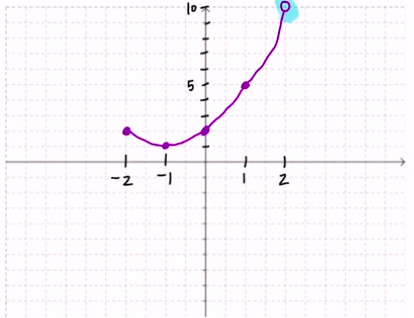
\includegraphics[width=0.4\textwidth]{/home/datura/niu/stats/stat128/lectures/1-4/figures/2.png} \\
            July 03, 2023  \\
           Computer Science \\
           Joliet Junior College \\
           United States\\
           
                
       \end{center}
    \end{titlepage}
    \tableofcontents
    \pagebreak \bigbreak \noindent
    \begin{center}
        \phantomsection
        \addcontentsline{toc}{section}{Chapter 5}
        \section*{Chapter 5}
    \end{center}
    \line(1,0){490}
    \bigbreak \noindent 
    \subsection{5.1: Probability Rules}
    \bigbreak \noindent 
    \textbf{\textit{\underline{Learning Objectives For This Section:}}}
    \begin{enumerate}
        \item \textbf{Understand Random Processes and the Law of Large Numbers}
        \item \textbf{Apply the Rules of Probabilities}
        \item \textbf{Compute and Interpret Probabilities Using the Empirical Method}
        \item \textbf{Compute and Interpret Probabilities Using the Classical Method}
        \item \textbf{Recognize and Interpret Subjective Probabilities}
    \end{enumerate}
    \bigbreak \noindent 
    \textbf{Vocab:}
    \begin{itemize}
        \item \textbf{Simulation:} is a technique used to recreate a random event.
        \item \textbf{Random Process:} represents scenarios where the outcome of any particular trial of an experiment is unknown, but the proportion (or relative frequency) of a particular outcome is observed and approaches a specific value
        \item \textbf{Probability:} Is the measure of the likelihood of a random phenomenon or chance behavior occurring. It deals with experiments that yield random short-term results or outcomes yet reveal long-term predictability. The long-term proportion in which a certain outcome is observed is the probability of that outcome. 
        \item \textbf{Outcomes:} Short term results
        \item \textbf{The Law of Large Numbers:} As the number of repetitions of a probability experiment increases, the proportion with which a certain outcome is observed gets closer to the probability of the outcome.
        \item \textbf{an experiment} is any process with uncertain results that can be repeated.
        \item \textbf{The sample space, $S$,} of a probability experiment is the collection of all possible outcomes for that experiment.
        \item \textbf{An event} is any collection of outcomes from a probability experiment. An event consists of one or more outcomes. We denote events with one outcome, sometimes called simple events, as $e_{i}$. In general, events are denoted using capital letters such as $ E$.
        \item \textbf{A probability model} lists the possible outcomes of a probability experiment and each outcome's probability. A probability model must satisfy Rules 1 and 2 of the rules of probabilities.
        \item  \textbf{An unusual event} is an event that has a low probability of occurring.
        \item An experiment has \textbf{equally likely outcomes} when each outcome has the same probability of occurring. 
        \item A \textbf{subjective probability} is a probability that is determined based on personal judgment.
    \end{itemize}

    \pagebreak \bigbreak \noindent
    \textbf{Formulas:}
    \begin{itemize}
        \item Computing probability with the empirical method
        \begin{align*}
            P(E) = \text{Relative frequency of E} = \frac{Frequency\ of\ E}{number\ of\ trials\ of\ experiment}
        .\end{align*}
        \item Computing Probability With The Classical Method
            \begin{itemize}
                \item If an experiment has n equally likely outcomes and if the number of ways that an event E can occur is m, then the probability of E,P(E), is
            \end{itemize}
            \begin{align*}
                P(E) = \frac{\text{number of ways that $E$ can occur}}{\text{number of possible outcomes}} = \frac{m}{n}
            .\end{align*}
            \begin{itemize}
                \item So, if S is the sample space of this experiment, then
                    \begin{align*}
                        P(E) = \frac{N(E)}{N(E)}
                    .\end{align*}
            where N(E) is the number of outcomes in E, and N(S) is the number of outcomes in the sample space.
            \end{itemize}
    \end{itemize}


    \pagebreak \bigbreak \noindent
    \textbf{\textit{\underline{Objective 1: Understand Random Processes and the Law of Large Numbers:}}}
    \bigbreak \noindent 
    Refer to vocab above for definition on the law of large numbers.
    \bigbreak \noindent 
    \qs{}{Brad and Allison have three girls. Brad tells Allison that he would like one more child because they are due to have a boy. What do you think of​ Brad's logic? }
    \bigbreak \noindent 
    Brad is incorrect due to the nonexistent Law of Averages. The fact that Brad and Allison had three girls in a row does not matter. The likelihood the next child will be a boy is about 0.5.

    \bigbreak \noindent 
    \begin{mdframed}
        \textbf{Example: A probability experiment consists of rolling a single six-sided fair die. A fair die is one in which each possible outcome is equally likely. For example, rolling a two is just as likely as rolling a five.}
      \bigbreak \noindent 
      \textbf{a.)  Identify the outcomes of the probability experiment. }
      \bigbreak \noindent 
      \textbf{b.) Identify the sample space}
      \bigbreak \noindent 
      \textbf{c.) Define the event $E$=“roll an even number”.}
      \bigbreak \noindent 
      \textbf{A.)} The outcomes from rolling a single fair die are $e_1=\text{``rolling a one''}=\{1\}$, $e_2=\text{``rolling a two''}=\{2\}$, $e_3=\text{``rolling a three''}=\{3\}$, $e_4=\text{``rolling a four''}=\{4\}$, $e_5=\text{``rolling a five''}=\{5\}$, and $e_6=\text{``rolling a six''}=\{6\}$.
      \bigbreak \noindent 
      \textbf{B.)} The set of all possible outcomes forms the sample space, $S=\{1,2,3,4,5,6\}$. There are six outcomes in the sample space.
      \bigbreak \noindent 
      \textbf{C.)} The event E=“roll an even number"$=\{2,4,6\}$.
    \end{mdframed}

    \bigbreak \noindent 
    \qs{}{If a person rolls a 6 sided dice and then flips a coin, describe the sample space of possible outcomes.
        \bigbreak \noindent 
        \textbf{Solution:}
        \bigbreak \noindent 
        The sample space is $\{1H,1T,2H,2T,3H,3T,4H,4T,5H,5T,6H,6T\}$
    }

    \pagebreak \bigbreak \noindent
    \textbf{\textit{\underline{Apply the Rules of Probabilities:}}}
    \bigbreak \noindent 
    In the following probability rules, the notation $P(E)$ means “the probability that event E occurs.”
    \bigbreak \noindent 
    \textbf{Rules of Probability:}
    \begin{enumerate}
        \item The probability of any event E, $P(E)$, must be greater than or equal to 0 and less than or equal to 1. That is, $0 \leq P(E) \leq 1$.
        \item The sum of the probabilities of all outcomes must equal 1. That is, if the sample space $S = \{e_1, e_2, \dots, e_n\}$, then
            \begin{align*}
                P(e_1) + P(e_2) + \dots + P(e_n) = 1.
            .\end{align*}
    \end{enumerate}
    \bigbreak \noindent 
    \begin{mdframed}
      \textbf{Example: Probability Model:}
      \bigbreak \noindent 
      In a bag of peanut candies, the colors of the candies can be brown, yellow, red, blue, orange, or green. Suppose that a candy is randomly selected from a bag. The table shows each color and the probability of drawing that color. Verify that this is a probability model.
      \bigbreak \noindent 
      \begin{center}
          \begin{center}
              \begin{tabular}{|l|c|}
              \hline
              Color & Probability \\
              	\hline
               	 Brown  & 0.12  \\
              	\hline
              	 Yellow & 0.15 \\
              	 \hline 
              	 Red & 0.12 \\
              	 \hline
              	 Blue & 0.23 \\
              	 \hline
              	 Orange & 0.23 \\
              	 \hline
              	 Green & 0.15 \\
              	 \hline
              \end{tabular}
          \end{center}
      \end{center}
      \bigbreak \noindent 
      \textbf{Solution:}
      \bigbreak \noindent 
        Rule 1 is satisfied because all probabilities are between 0 and 1, inclusive.
          \bigbreak \noindent 
          Rule 2 is satisfied because $\sum P(E)= 1$
    \end{mdframed}

    \bigbreak \noindent 
    \textbf{Key Concepts Regarding Probabilities}
    \bigbreak \noindent 
    \begin{itemize}
        \item If an event is impossible, the probability of the event is 0.
        \item If an event is a certainty, the probability of the event is 1.
        \item The closer a probability is to 1, the more likely the event will occur.
        \item The closer a probability is to 0, the less likely the event will occur.
        \item For example, an event with probability 0.8 is more likely to occur than an event with probability 0.75.
        \item An event with probability 0.8 will occur about 80 times out of 100 repetitions of the experiment, whereas an event with probability 0.75 will occur about 75 times out of 100.
    \end{itemize}

    \pagebreak \bigbreak \noindent
    \qs{}{In a certain card​ game, the probability that a player is dealt a particular hand is 0.46 . Explain what this probability means. If you play this card game 100​ times, will you be dealt this hand exactly  ​ 46 times? Why or why​ not?
        \bigbreak \noindent 
        \textbf{Solution:}
        \bigbreak \noindent 
        The probability  0.46 means that approximately  46 out of every 100 dealt hands will be that particular hand.​ No, you will not be dealt this hand exactly 46 times since the probability refers to what is expected in the​ long-term, not​ short-term.
    }

    \bigbreak \noindent \bigbreak \noindent 
    \textbf{Unusual Event}
    \bigbreak \noindent 
    Typically, an event with a probability less than 0.05 (or 5\%) is considered unusual, but this cutoff point is not set in stone. The researcher and the context of the problem determine the probability that separates unusual events from not so unusual events.

    \bigbreak \noindent \bigbreak \noindent 
    \textbf{The three methods for determining the probability of an event:}
    \bigbreak \noindent 
    \begin{itemize}
        \item the Empirical Method
        \item the Classical Method
        \item the Subjective Method
    \end{itemize}

    \bigbreak \noindent 
    \textbf{Approximating Probabilities Using the Empirical Approach:}
    \bigbreak \noindent 
    The probability of an event E occurring is approximately the number of times event E is observed divided by the number of repetitions (or trials) of the experiment.
    \begin{align*}
        P(E) = \text{Relative frequency of E} = \frac{Frequency\ of\ E}{number\ of\ trials\ of\ experiment}
    .\end{align*}

    \bigbreak \noindent 
    \nt{When we find probabilities using the empirical approach, the result is approximate because different trials of the experiment lead to different outcomes and, therefore, different estimates of $P(E)$}

    \bigbreak \noindent 
    Surveys are probability experiments. Why? Each time a survey is conducted, a different random sample of individuals is selected. Therefore, the results of a survey are likely to be different each time the survey is conducted because different people are included.
    \pagebreak \bigbreak \noindent
    \textbf{\textit{\underline{Compute and Interpret Probabilities Using the Classical Method}}}
    \bigbreak \noindent 
    The empirical method gives an approximate probability of an event by conducting a probability experiment. The classical method of computing probabilities does not require that a probability experiment actually be performed. Rather, it relies on counting techniques.
    \bigbreak \noindent 
    The classical method of computing probabilities requires equally likely outcomes. An experiment has equally likely outcomes when each outcome has the same probability of occurring. For example, when a fair die is thrown once, each of the six outcomes in the sample space, {1,2,3,4,5,6}, has an equal chance of occurring
     Computing Probability With The Classical Method
     \bigbreak \noindent 
     If an experiment has n equally likely outcomes and if the number of ways that an event E can occur is m, then the probability of E,P(E), is
    \begin{align*}
        P(E) = \frac{\text{number of ways that $E$ can occur}}{\text{number of possible outcomes}} = \frac{m}{n}
    .\end{align*}
    \bigbreak \noindent 
         So, if S is the sample space of this experiment, then
            \begin{align*}
                P(E) = \frac{N(E)}{N(E)}
            .\end{align*}
    where N(E) is the number of outcomes in E, and N(S) is the number of outcomes in the sample space.

    \bigbreak \noindent \bigbreak \noindent 
    \textbf{Comparing Empirical Probabilities and Classical Probabilities}
    \bigbreak \noindent 
    We just saw that the classical probability of rolling a seven is 16≈0.167. Suppose a pit boss at a casino rolls a pair of dice 100 times and obtains 15 sevens. From this empirical evidence, we would assign the probability of rolling a seven as 15100=0.15. If the dice are fair, we would expect the relative frequency of sevens to get closer to 0.167 as the number of rolls of the dice increases. In other words, the empirical probability will get closer to the classical probability as the number of trials of the experiment increases due to the Law of Large Numbers. If the two probabilities do not get closer, we may suspect that the dice are not fair.
    \bigbreak \noindent 
    \nt{In simple random sampling, each individual has the same chance of being selected. Therefore, we can use the classical method to compute the probability of obtaining a specific sample.}

    \bigbreak \noindent \bigbreak \noindent 
    \textbf{\textit{\underline{Recognize and Interpret Subjective Probabilities}}}
    \bigbreak \noindent 
    If a sports reporter is asked what he thinks the chances are for the Boston Red Sox to play in this season's World Series, the reporter would likely process information about the Red Sox (pitching staff, leadoff hitter, and so on) and then make an educated guess of the likelihood. The reporter may respond that there is a 20\% chance the Red Sox will play in the World Series. This forecast is a probability, although it is not based on relative frequencies. We cannot, after all, repeat the experiment of playing a season under the same circumstances (same players, schedule, and so on) over and over. Nonetheless, the forecast of 20\%=0.20 does satisfy the criterion that a probability be between 0 and 1, inclusive. This forecast is known as a subjective probability.
    \bigbreak \noindent r
    Subjective probabilities are legitimate and are often the only method of assigning likelihood to an outcome. For instance, a financial reporter may ask an economist about the likelihood of the economy falling into recession next year. Again, we cannot conduct an experiment n times to find a relative frequency. The economist must use knowledge of the current conditions of the economy and make an educated guess about the likelihood of recession.

    \pagebreak \bigbreak \noindent
    \subsection{5.2: The Addition Rule and Complements}
    \bigbreak \noindent 
    \textbf{\textit{\underline{Learning Objectives For This Section:}}}
    \begin{enumerate}
      \item \textbf{Use the Addition Rule for Disjoint Events}
      \item \textbf{Use the General Addition Rule}
      \item \textbf{Compute the Probability of an Event Using the Complement Rule}
    \end{enumerate}
    \bigbreak \noindent 
    \textbf{Vocab:}
    \begin{itemize}
      \item \textbf{Disjoint:} Two events are disjoint if they have no outcomes in common. 
      \item \textbf{Mutually Exclusive:} Another name for disjoint events.
        \item \textbf{Complement of $E$:} Let $S$ denote the sample space of a probability experiment and let $E$ denote an event. The complement of $E $, denoted $E^{C} $, is all outcomes in the sample space $S $ that are not outcomes in the event $E $.
    \end{itemize}
    \bigbreak \noindent 
    \textbf{Formulas:}
    \begin{itemize}
        \item Addition Rule for Disjoint Events:
            \begin{itemize}
                \item if $E $ and $F $ are disjoint (or mutually exclusive) events, then:
                    \begin{align*}
                        P(E\ or\ F) = P(E) + P(F)
                    .\end{align*}
            \end{itemize}
        \item Complement Rule:
            \begin{itemize}
                \item If $E$ represents any event and $E^{C}$ represents the complement of E, then
            \end{itemize}
            \begin{align*}
                P(E^{C}) = 1-P(E)                
            .\end{align*}
    \end{itemize}

    \pagebreak \bigbreak \noindent
    \textbf{\textit{\underline{Use the Addition Rule for Disjoint Events}}}
    \thmcon{\textbf{\textit{\underline{Definition: Addition Rule for Disjoint Events}}}
    \bigbreak \noindent
    If $E $ and $F $ are disjoint (or mutually exclusive) events, then:
    \begin{align*}
        P(E\ or\ F) = P(E) + P(F)
    .\end{align*}
    } 
    \bigbreak \noindent 
    We often draw  pictures of events using \textbf{Venn Diagrams}. These pictures represent events as circles enclosed in a rectangle. The
    rectangle represents the sample space, and each circle represents an event. For example, suppose we randomly select a 
    chip from a bag where each chip in the bag is labeled 0,1,2,3,4,5,6,7,8,9. Let $E $ represent the event "Choose a number less than or equal to 2",
    and let $F $ represent the event "Choose a number greater than or equal to 8." These events are disjoint as shown in the figure.
    \bigbreak \noindent 
    \textit{Figure:}
    % \begin{figure}[ht]
    %     \centering
    %     \incfig{figab}
    %     \label{fig:figab}
    % \end{figure}
    \bigbreak \noindent 
    So you can see that these events are \textbf{Disjoint} because they \textbf{do not} share any outcomes.
    \bigbreak \noindent 
    We can then compute the probability of event $E$ using the classical approach
    \begin{align*}
        P(E) = \frac{N(E)}{N(S)} = \frac{3}{10} = 0.3
    .\end{align*}
    \bigbreak \noindent 
    Similarly,  if we wanted to know the probability of event $F$: 
    \begin{align*}
        P(F) = \frac{N(F)}{N(S)} = \frac{2}{10} = 0.2
    .\end{align*}
    \bigbreak \noindent 
    What if we wanted to know the probability of $E$ \textbf{or} $F $? ($P(E\ or\ F)$):
    \begin{align*}
        P(E\ or\ F) = \frac{N(E\ or\ F)}{N(S)} = \frac{5}{10} = 0.5 
    .\end{align*}
    \bigbreak \noindent 
    However, we can use the \textbf{Addition Rule}, which goes like:
    \begin{align*}
     P(E\ or\ F) = P(E) + P(F) = 0.3 + 0.2  \\
     = 0.5
    .\end{align*}

    \pagebreak \bigbreak \noindent
    \textbf{\textit{\underline{Compute the Probability of an Event Using the Complement Rule}}}
    \bigbreak \noindent 
    Suppose that the probability of an event $E $ is known and we would like to determine the probability that $E $ does not occur. This can be accomplished using the idea of complements.
    \bigbreak \noindent 
    Because $E$ and $E^{C}$ are mutually exclusive,
    \thmcon{\textbf{\textit{\underline{Definition:}}}
    \bigbreak \noindent
     \textbf{Complement Rule:}
    \begin{itemize}
        \item If $E$ represents any event and $E^{C} $ represents the complement of $E$, then
    \end{itemize}
    \begin{align*}
        P(E^{C}) = 1-P(E)                
    .\end{align*}

    }
    \bigbreak \noindent 
      \textbf{Example: Compliment Rule}
      \bigbreak \noindent 
      Suppose 31.6\% of American households own a dog. What is the probability that a randomly selected household \textbf{does} not own a dog?
      \begin{align*}
          P(E^{C}) = 1 - P(E) \\
          = 1- 0.36 \\
          =0.684
      .\end{align*}
    \bigbreak \noindent 
      \textbf{Example: Compliment Rule:}
      \bigbreak \noindent 
      Let:
      \begin{align*}
          S=\{9,10,11,12,13,14,15,16,17,18,19,20\} \\
          E=\{11,12,13,14,15,16,17,18,19\}
      .\end{align*}
      Assume each outcome is equally likely. List the outcomes in $E^{C} $ Find $P(E^{C})$
      \begin{align*}
          P(E) = \frac{9}{12} = \frac{3}{4} = 0.75 \\
          P(E^{C}) =1- 0.75 \\
          = 0.25
      .\end{align*}

    \pagebreak \bigbreak \noindent
    \subsection{ 5.3: Independence and the Multiplication Rule}
    \bigbreak \noindent 
    \textbf{\textit{\underline{Learning Objectives For This Section:}}}
    \begin{enumerate}
        \item \textbf{Identify Independent Events}
        \item \textbf{Compute At-least Probabilities}
        \item \textbf{Use the Multiplication Rule for Independent Events}
    \end{enumerate}
    \bigbreak \noindent 
    \textbf{Vocab:}
    \begin{itemize}
        \item \textbf{Two events being Independent: } Two events $E$ and $F$ are independent if the occurrence of event $E$ in a probability experiment does not affect the probability of event $F $.
        \item \textbf{Two events being Dependent:} Two events are dependent if the occurrence of event $E $ in a probability experiment affects the probability of event $F$.
    \end{itemize}
    \bigbreak \noindent 
    \textbf{Formulas:}
    \begin{itemize}
        \item If $E$ and $F$ are independent events, then
    \begin{align*}
         P(E \text{ and } F) = P(E) \cdot P(F) 
    .\end{align*}
    \bigbreak \noindent 
    \item If $E_1, E_2, E_3, \ldots, E_n$ are independent events, then
    \begin{align*}
         P(E_1 \text{ and } E_2 \text{ and } E_3 \text{ and } \ldots \text{ and } E_n) = P(E_1) \cdot P(E_2) \cdot \ldots \cdot P(E_n)
    .\end{align*}

        
    \end{itemize}
    \pagebreak \bigbreak \noindent
    \textbf{\textit{\underline{Identify Independent Events}}}
    \bigbreak \noindent 
    \textbf{Example A:} Suppose you draw a card from a standard 52-card deck of cards and then roll a die. The events "draw a heart" and "roll a number" are \textbf{independent} because the results of choosing a card do not impact the results of the die toss.
    \bigbreak \noindent 
    \textbf{Example B:} Suppose two 40-year old women who live in the United States are randomly selected. The events "woman 1 survived the year" and "women 2 survives the year" are \textbf{independent}
    \bigbreak \noindent 
    \textbf{Example C:} Suppose two 40-year old women live in the same apartment complex. The events "woman 1 survived the year" and "women 2 survives the year" are \textbf{dependent}
      
    \bigbreak \noindent 
    \nt{When we take small samples from large finite populations, we make the assumption of independence even though the events are technically dependent.
        \bigbreak \noindent 
        As a general rule of thumb, if the sample size $n $ is no more than 5\% of the population $N $ ($n \leq 0.05 N $), we assume independence.

    }

    \bigbreak \noindent 
    \qs{}{Determine whether the events E and F are independent or dependent. Justify your answer.
        \bigbreak \noindent 
        \begin{center}
            E: A person having an at-fault accident \\
            F: The same person being prone to road rage
        \end{center}
        \bigbreak \noindent 
        \textbf{Solution:}
        E and F are dependent because  being prone to road rage can affect the probability of a person having an at-fault accident
        \bigbreak \noindent 
        \begin{center}
            E: A randomly selected person coloring her hair black. \\
            F: A different randomly selected person coloring her hair blond.
        \end{center}
        \bigbreak \noindent 
        \textbf{Solution:}
        E cannot affect F and vice versa because the people were randomly​ selected, so the events are independent.
        \bigbreak \noindent 
        \begin{center}
            E: The rapid spread of a cocoa plant disease \\
            F: The price of chocolate
        \end{center}
        \bigbreak \noindent 
        \textbf{Solution:}
        \text{The rapid spread of a cocoa plant disease could affect the price of chocolate, so } $\mathrm{E}$ \text { and } $\mathrm{F}$ \text {are dependent.}

}
    \pagebreak \bigbreak \noindent
    \textbf{ Disjoint (or Mutually Exclusive) Events versus Independent Events}
    \bigbreak \noindent 
    Disjoint events and independent events are different concepts.
    \begin{itemize}
        \item Recall that two events are disjoint if they have no outcomes in common, that is, if knowing that one of the events occurs, we know that the other event did not occur.
        \item Independence means that one event occurring does not affect the probability of the other event occurring.
    \end{itemize}
    \bigbreak \noindent 
    Therefore, knowing that two events are disjoint means that the events are not independent.
    \bigbreak \noindent 
    Consider the experiment of rolling a single die. Let $E$ represent the event "roll an even number" and let $F$ represent the event "roll an odd number." We can see that $E$ and $F$ are disjoint (mutually exclusive) because they have no outcomes in common. In addition, $P(E)=\frac{1}{2}$ and $P(F)=\frac{1}{2}$. However, if we are told that the roll of the die is going to be an even number, then what is the probability of event $F$? Because the outcome will be even, the probability of event $F$ is now 0 (and the probability of event $E$ is now 1). So knowledge of event $E$ changes the likelihood of observing event $F$.

    \bigbreak \noindent \bigbreak \noindent 
    \textbf{\textit{\underline{Use the Multiplication Rule for Independent Events}}}
    \bigbreak \noindent 
    Suppose that you flip a fair coin twice. What is the probability that you obtain a head on both flips, that is, a head on the first flip and a head on the second flip? If $H$ represents the outcome "heads" and $T$ represents the outcome "tails," then the sample space of this experiment is
    \begin{align*}
        S={HH,HT,TH,TT}
    .\end{align*}
    \bigbreak \noindent 
    There is one outcome with both heads. Because each outcome is equally likely, we have
    \begin{align*}
        P(\text{heads on Flip 1 and heads on Flip 2})=\frac{N(\text{heads on Flip 1 and heads on Flip 2})}{N(S)} \\ =\frac{1}{4}
    .\end{align*}
    \bigbreak \noindent 
    We may have intuitively figured this out by recognizing $P(\text{head})=\frac{1}{2}$ for each flip. So it seems reasonable that
    \begin{align*}
        P(\text{heads on Flip 1 and heads on Flip 2})=P(\text{heads on Flip 1})\cdot P(\text{heads on Flip 2})\\ =\frac{1}{2}\cdot\frac{1}{2}\\ =\frac{1}{4}
    .\end{align*}
    \bigbreak \noindent 
    Because both approaches result in the same answer, we conjecture that $P(E \text{ and } F)=P(E)\cdot P(F)$, which is true.
    \pagebreak \bigbreak \noindent
    \thmcon{\textbf{\textit{\underline{Definition: Multiplication Rule for Independent Events}}}
    \bigbreak \noindent
    If $E$ and $F$ are independent events, then
    \begin{align*}
         P(E \text{ and } F) = P(E) \cdot P(F) 
    .\end{align*}
    \bigbreak \noindent 
    If $E_1, E_2, E_3, \ldots, E_n$ are independent events, then
    \begin{align*}
         P(E_1 \text{ and } E_2 \text{ and } E_3 \text{ and } \ldots \text{ and } E_n) = P(E_1) \cdot P(E_2) \cdot \ldots \cdot P(E_n)
    .\end{align*}
    }
    \bigbreak \noindent \bigbreak \noindent 
    \qs{}{Suppose that events $E$  $F$ are independent,  $P(E)=0.6$ and $P(F)=0.7$ What is the $P(E\ and\ F)$?
        \bigbreak \noindent 
        \begin{align*}
            P(E\ and\ F)  = P(E) \cdot P(F) = 0.6 \cdot 0.7 = 0.42
        .\end{align*}
    }

    \bigbreak \noindent \bigbreak \noindent 
    \textbf{\textit{\underline{Compute At-least Probabilities}}}
    \bigbreak \noindent 
    Usually, when computing probabilities involving the phrase at least, use the Complement Rule.
    \bigbreak \noindent 
    The phrase at least means “greater than or equal to.” For example, a person must be at least 17 years old to see an R-rated movie. This means that the person's age must be greater than or equal to 17 to watch the movie.
    \bigbreak \noindent \bigbreak \noindent 
    \qs{}{The probability that a randomly selected female aged 60 years will survive the year is 0.99186 according to the National Vital Statistics Report. What is the probability that at least one of 500 randomly selected 60-year-old females will die during the course of the year?
        \bigbreak \noindent 
        \textbf{Solution:}
        \bigbreak \noindent 
        The phrase at least means “greater than or equal to,” so we want to know the probability that 1 or 2 or 3 or ⋯ or 500 60-year-old females will die during the year. These events are mutually exclusive, so
        \begin{align*}
            P(1 \text{ or } 2 \text{ or } 3 \text{ or } \dots \text{ or } 500 \text{ die}) &= P(1 \text{ dies}) + P(2 \text{ dies}) + P(3 \text{ dies}) + \dots + P(500 \text{ dies})
        .\end{align*}
        Computing these probabilities would be very time-consuming. However, notice that the complement of “at least one dying” is “none die”, or all 500 survive. Use the Complement Rule to compute the probability.
        \bigbreak \noindent 
        So:
        \begin{align*}
            P(\text{at least one dies}) = 1- P(\text{None dies}) \\
            = 1 - (0.99186)^{500} \\
            = 0.9832
        .\end{align*}
    }

    \pagebreak 
    \begin{center}
        \phantomsection
        \addcontentsline{toc}{section}{Chapter 6}
        \section*{Chapter 6}
    \end{center}
    \line(1,0){490}
    \bigbreak \noindent 
    \phantomsection
    \addcontentsline{toc}{subsection}{6.1: Discrete Random Variables}
    \subsection*{6.1: Discrete Random Variables}
    \bigbreak \noindent 
    \textbf{\textit{\underline{Learning Objectives For This Section:}}}
    \begin{enumerate}
        \item \textbf{Distinguish between Discrete and Continuous Random Variables}
        \item \textbf{Identify Discrete Probability Distributions}
        \item \textbf{Graph Discrete Probability Distributions}
        \item \textbf{Compute and Interpret the Mean of a Discrete Random Variable}
        \item \textbf{Interpret the Mean of a Discrete Random Variable as an Expected Value}
        \item \textbf{Compute the Standard Deviation of a Discrete Random Variable}
    \end{enumerate}
    \bigbreak \noindent 
    \textbf{Vocab:}
    \begin{itemize}
        \item A \textbf{random variable} is a numerical measure of the outcome of a probability experiment; so its value is determined by chance.
        \begin{itemize}
            \item Random variables are typically denoted using capital letters such as $X$ 
        \end{itemize}
        \item A \textbf{discrete random variable} has either a finite or countable number of values. The values of a discrete random variable can be plotted on a number line with space between each point. See Figure 1(a).
        \item A \textbf{continuous random variable} has infinitely many values. The values of a continuous random variable can be plotted on a line in an uninterrupted fashion. See Figure 1(b).
        \item The \textbf{probability distribution} of a discrete random variable X provides the possible values of the random variable and their corresponding probabilities. A probability distribution can be in the form of a table, graph, or mathematical formula.
        \item Because the mean of a random variable represents what we would expect to happen in the long run, it is also called the \textbf{expected value}, $E(X)$. The interpretation of the expected value is the same as the interpretation of the mean of a discrete random variable.
    \end{itemize}
    \pagebreak \bigbreak \noindent 
    \textbf{Formulas:}
    \begin{itemize}
        \item \textbf{Notation for probability of discrete random variables}
            \begin{align*}
                P(X)
            .\end{align*}
            \begin{itemize}
                \item Read as:
                    \begin{center}
                        "The probability that the random variable $X $ equals $x $"
                    \end{center}
            \end{itemize}
        \item \textbf{Mean of a Discrete Random Variable}
            \begin{align*}
                \mu_X = \summation{n}{i=1}\ \  x \cdot P(x)
            .\end{align*}
            Where $x $ is the value of the random variable and $P(x)$ is the probability of observing the value $x$.
        \item \textbf{Expected Value:}
            \begin{align*}
                E(X) = \mu_{X}
            .\end{align*}
        \item \textbf{Standard Deviation of a Discrete Random Variable}
            \begin{align*}
                \sigma_X = \sqrt{\sum [(x - \mu_X)^2 \cdot P(x)]}
            .\end{align*}
        Where $x$ is the value of the random variable, $\mu_X$ is the mean of the random variable, and $P(x)$ is the probability of observing $x$.
        \item \textbf{Variance of discrete random variable:}
            \begin{align*}
                \mu^{2}
            .\end{align*}
    \end{itemize}
    \pagebreak \bigbreak \noindent 
    \textbf{\textit{\underline{Distinguish between Discrete and Continuous Random Variables}}}
    \bigbreak \noindent 
    \begin{enumerate}[label=(\alph*)]
        \item The number of A's earned in a section of statistics with 15 students enrolled is a discrete random variable because its value results from counting. If the random variable $X$ represents the number of A's, then the possible values of $X$ are $x = 0, 1, 2, \ldots, 15$.
        \item The number of cars that travel through a McDonald's drive-through in the next hour is a discrete random variable because its value results from counting. If the random variable $X$ represents the number of cars, the possible values of $X$ are $x = 0, 1, 2, \ldots$. That is, the number of cars can be any whole number, and we do not impose an upper limit on the number of cars.
        \item The speed of the next car that passes a state trooper is a continuous random variable because speed is measured. If the random variable $S$ represents the speed, the possible values of $S$ are all positive real numbers; that is, $s > 0$. Even though a radar gun may report the speed of a car as 37 miles per hour, it is actually any number greater than or equal to 36.5 mph and less than 37.5 mph. That is, $36.5 \leq s < 37.5$.
    \end{enumerate}

    \bigbreak \noindent \bigbreak \noindent 
    \textbf{\textit{\underline{Identify Discrete Probability Distributions}}}
    \bigbreak \noindent 
    \textbf{Rules for a Discrete Probability Distribution:}
    \bigbreak \noindent 
    Let $P(x)$ denote the probability that the random variable $X$ equals $x$; then
    \begin{itemize}
        \item $ \sum P(x) = 1 $
        \item $0 \leq P(x) \leq 1$
    \end{itemize}

    \bigbreak \noindent \bigbreak \noindent 
    \textbf{\textit{\underline{Graph Discrete Probability Distributions}}}
    \bigbreak \noindent 
    In the graph of a discrete probability distribution, the horizontal axis is the value of the discrete random variable and the vertical axis is the corresponding probability of the discrete random variable. When graphing a discrete probability distribution, we want to emphasize that the data are discrete. Therefore, draw the graph of discrete probability distributions using vertical lines above each value of the random variable to a height that is the probability of the random variable.
    \bigbreak \noindent 
    \textit{Discrete Probability Distribution Figure:}
    % \begin{figure}[ht]
    %     \centering
    %     \incfig{enumab}
    %     \label{fig:enumab}
    % \end{figure}

    \pagebreak \bigbreak \noindent 
    \textbf{Distribution Shape of Discrete Probability Distributions}
    \bigbreak \noindent 
    Graphs of discrete probability distributions help determine the shape of the distribution.
    \bigbreak \noindent 
    Recall that we describe distributions as skewed left, skewed right, or symmetric. The graph in Figure 2 is skewed left.

    \bigbreak \noindent \bigbreak \noindent 
    \textbf{\textit{\underline{Compute and Interpret the Mean of a Discrete Random Variable}}}
    \bigbreak \noindent 
    \textbf{Finding Mean of a Discrete Random Variable In Statcrunch:}
    \begin{enumerate}
        \item Stat $> $ Calculators $> $ Custom
        \item Select Values in:
        \item Select Weights in (P(X)):
        \item Compute
    \end{enumerate}
    \bigbreak \noindent \bigbreak \noindent 
    \textbf{How to Interpret the Mean of a Discrete Random Variable}
    \bigbreak \noindent 
    The mean of a discrete random variable can be thought of as the mean outcome of the probability experiment if we repeated the experiment many times. 
    \bigbreak \noindent 
    As the number of repetitions of the experiment increases... The mean value of the $n $ trials will approach $\mu_{X}$ (The difference between $\overline{x} $ and $\mu_{X} $ gets closer to 0 as $n$ increases)

    \pagebreak \bigbreak \noindent 
    \textbf{\textit{\underline{Interpret the Mean of a Discrete Random Variable as an Expected Value}}}
    \bigbreak \noindent 
    \begin{mdframed}
      \textbf{Example: A term life insurance policy will pay a beneficiary a certain sum of money upon the death of the policy holder. These policies have premiums that must be paid annually. Suppose a life insurance company sells a \$250,000 one-year term life insurance policy to a 49-year-old female for \$530. According to the National Vital Statistics Report, Vol. 47, No. 28, the probability that the female will survive the year is 0.99791. Compute the expected value of this policy to the insurance company.}
      \bigbreak \noindent 
      \textbf{Approach:}
      \bigbreak \noindent 
      The experiment has two possible outcomes: survival or death. Let the random variable X represent the payout (money lost or gained), depending on survival or death of the insured. Assign probabilities to each payout and substitute these values into $\mu_{X} = \sum (x \cdot P(X)) $
      \bigbreak \noindent 
      \textbf{Step 1}. Because $P(\text{survives}) = 0.99791$, $P(\text{dies}) = 0.00209$. If the client survives the year, the insurance company makes \$530, or $x = +530$. If the client dies during the year, the insurance company must pay \$250,000 to the client's beneficiary, but still keeps the \$530 premium; so $x = \$530 - \$250,000 = -\$249,470$. The value is negative because it is money paid by the insurance company. The probability distribution is listed in Table 3.
      \begin{center}
          \begin{center}
              \begin{tabular}{|l|c|}
              \hline
              $x$ & $ P(X)$ \\
              	\hline
               	\$530 (survives)  & 0.99791  \\
              	\hline
              	-\$249,470 (dies) &0.00209 \\
              	\hline
              \end{tabular}
          \end{center}
      \end{center}
      \bigbreak \noindent 
      \textbf{Step 2.} The expected value (from the point of view of the insurance company) of the policy is
      \begin{align*}
          E(X) = \mu_{X} \\
          = \sum (x \cdot P(X)) \\
          = (\$530 \cdot 0.99791) + (-\$249470 \cdot 0.00209) \\
          = \$7.50
      .\end{align*}
      \bigbreak \noindent 
      \textbf{Therefore:}
      \bigbreak \noindent 
      The company expects to make \$7.50 for each 49-year-old female client it insures. The \$7.50 profit of the insurance company is a long-term result. It does not make \$7.50 on each 49-year-old female it insures; rather, the average profit per 49-year-old female insured is \$7.50. Because this is a long-term result, the insurance "idea" will not work with only a few insured.
      \end{mdframed}


      \pagebreak \bigbreak \noindent 
      \textbf{\textit{\underline{Compute the Standard Deviation of a Discrete Random Variable}}}
      \bigbreak \noindent 
      \textbf{Statcrunch Steps:}
      \begin{enumerate}
          \item Stat $> $ Calculators $> $ Custom
        \item Select Values in:
        \item Select Weights in (P(X)):
        \item Compute
      \end{enumerate}

      \pagebreak 
        \phantomsection
        \addcontentsline{toc}{subsection}{6.2: The Binomial Probability Distribution}
        \subsection*{6.2: The Binomial Probability Distribution}
      \bigbreak \noindent 
      \textbf{\textit{\underline{Learning Objectives For This Section:}}}
      \begin{enumerate}
            \item \textbf{Determine Whether a Probability Experiment is a Binomial Experiment}
          \item \textbf{Compute Probabilities of Binomial Experiments}
          \item \textbf{Compute the Mean and Standard Deviation of a Binomial Random Variable}
          \item \textbf{Graph a Binomial Probability Distribution}
      \end{enumerate}
      \bigbreak \noindent 
      \textbf{Vocab:}
      \begin{itemize}
          \item The \textbf{binomial probability distribution} is a discrete probability distribution that describes probabilities for experiments in which there are two mutually exclusive (disjoint) outcomes. These two outcomes are generally referred to as success (such as making a free throw) and failure (such as missing a free throw). Experiments in which only two outcomes are possible are referred to as binomial experiments, provided that certain criteria are met.
          \item \textbf{A combination} is a collection, without regard to order and without repetition, in which  $r $  objects are chosen from  n  distinct objects with  $r \leq n $.
        \item \textbf{Trial:} Each repetition of the experiment. 

      \end{itemize}
      \bigbreak \noindent 
      \textbf{Formulas:}
      \begin{itemize}
          \item \textbf{nCk (Combinations):}
              \begin{itemize}
                  \item The  $n$  objects are distinct
                  \item Repetition of objects is not allowed, and
                  \item Order is not important
              \end{itemize}
              \begin{align*}
                  nCk = \frac{n!}{(k!(n-k)!)}
              .\end{align*}
            \item \textbf{Binomial Probability Distribution Function}
                \begin{align*}
                    P(x) = \binom{n}{x} \cdot p^x \cdot (1 - p)^{n-x}, \quad x = 0, 1, 2, \ldots, n
                .\end{align*}
                where $p$ is the probability of success.
            \item \textbf{Mean (or Expected Value) and Standard Deviation of a Binomial Random Variable}
                \begin{itemize}
                    \item A binomial experiment with n independent trials and probability of success p has mean, $\mu_X$, and standard deviation, $\sigma_X$, given by the formulas
                \end{itemize}
                \begin{align*}
                    \mu_X = np,\ \text{and standard deviation,}\ \sigma_X = \sqrt{np(1-p)}
                .\end{align*}
      \end{itemize}

      \pagebreak \bigbreak \noindent 
      \textbf{\textit{\underline{Determine Whether a Probability Experiment Is a Binomial Experiment}}}
      \bigbreak \noindent 
      \textbf{Critera:}
      \bigbreak \noindent 
      An experiment is said to be a \textbf{binomial experiment} if:
      \begin{enumerate}
          \item The experiment is preformed a fixed number of times. Each repetition of the experiment is called a \textbf{trial}
            \item The trials are independent. This means that the outcome of one trial will not affect the outcome of the other trials.
            \item for each trial, there are two mutually exclusive outcomes, success or failure.
            \item The probability of success is fixed for each trial of the experiment.
      \end{enumerate}

      \bigbreak \noindent \bigbreak \noindent 
      \textbf{Notation used in the binomial probability distribution:}
      \begin{itemize}
          \item There are $n $ independent trials of the experiment.
        \item let $p $ denote the probability of success so that $1-p $ is the probability of failure
        \item Let $X $ be a binomial random variable that denotes the number of successes in $n $ independent trials of the experiment. So $0 \leq X \leq n $
      \end{itemize}

      \bigbreak \noindent \bigbreak \noindent 
      \textbf{\textit{\underline{Compute Probabilities of Binomial Experiments}}}
      \bigbreak \noindent 
      Now we will compute probabilities for a binomial random variable $X$. We present three methods for obtaining binomial probabilities:
      \bigbreak \noindent 
      \begin{enumerate}
          \item The binomial probability distribution formula
          \item A table of binomial probabilities
          \item Technology
      \end{enumerate}
      \bigbreak \noindent 

      \bigbreak \noindent \bigbreak \noindent 
      \textbf{Using the Binomial Probability Distribution Function in Statcrunch}
      \bigbreak \noindent 
      \textbf{Steps:}
      \begin{enumerate}
          \item Stat $> $ Calculators $> $ Binomial
        \item Enter $n $
        \item Enter $p $
        \item Enter info for $P(X)$
        \item Compute
      \end{enumerate}

      \pagebreak \bigbreak \noindent 
      \textbf{\textit{\underline{Compute the Mean and Standard Deviation of a Binomial Random Variable}}}
      \bigbreak \noindent 
      \begin{mdframed}
        \textbf{Example: According to CTIA, 55\% of all U.S. households are wireless-only households. In a simple random sample of 500 households, determine the mean and standard deviation number of wireless-only households. Compute the mean and std. dev}
        \bigbreak \noindent 
        \textbf{Approach:}
        \bigbreak \noindent 
        This is a binomial experiment with $n = 500$ and $p = 0.55$. Using $\mu_X = np$, we can find the mean as $\mu_{x} = \sqrt{np(1-p)} $
        \bigbreak \noindent 
        \textbf{Solution:}
        \bigbreak \noindent 
        \begin{align*}
            \mu_X = np = 500(0.55) = 275 \quad \\ \text{and} \\ \quad \sigma_X = \sqrt{np(1-p)} = \sqrt{500(0.55)(1-0.55)} = \sqrt{123.75} \\ \approx 11.1
        .\end{align*}

      \end{mdframed}

      \bigbreak \noindent \bigbreak \noindent 
      \textbf{\textit{\underline{Graph a Binomial Probability Distribution}}}
      \bigbreak \noindent 
      To graph a binomial probability distribution, first find the probabilities for each possible value of the random variable. Then follow the same approach as was used to graph discrete probability distributions.
      \bigbreak \noindent 
      \textbf{Shape of Binomial Probability Distribution for Various Values of $p $ }
      \bigbreak \noindent 
      The binomial probability distribution is
      \begin{itemize}
          \item skewed right if $p <0.5$
          \item symmetric and approximately bell-shaped if $p=0.5$
          \item skewed left of $p>0.5$ 
      \end{itemize}

      \bigbreak \noindent \bigbreak \noindent 
      \textbf{Shape of the Graph of a Binomial Probability Distribution for Various Values of $n $ }
      \bigbreak \noindent 
      \begin{itemize}
          \item For a fixed $p$, as the number of trials $n $ in a binomial experiment increases, the probability distribution of the random variable $X$ becomes bell-shaped.
          \item As a rule of thumb, if $np(1−p) \geq 10$, the probability distribution will be approximately bell-shaped.
      \end{itemize}
      \bigbreak \noindent 
      \nt{This result allows us to use the Empirical Rule to identify unusual observations in a binomial experiment. Recall that the Empirical Rule states that in a bell-shaped distribution, about 95\% of all observations lie within 2 standard deviations of the mean. That is, about 95\% of the observations lie between μ−2σ and μ+2σ. Any observation that lies outside this interval may be considered unusual because the observation occurs less than 5\% of the time.}

      \pagebreak 
      \bigbreak \noindent 
      \begin{mdframed}
        \textbf{Example: According to CTIA, 55\% of all U.S. households are wireless-only. In a simple random sample of 500 households, 301 were wireless-only. Is this result unusual?}
        \bigbreak \noindent 
        \textbf{Approach:}
        \bigbreak \noindent 
        Because $np(1-p) = 500(0.55)(1-0.55) = 123.75 \geq 10$, the binomial probability distribution is approximately bell-shaped. Therefore, we can use the Empirical Rule: If the observation is less than $\mu - 2\sigma$ or greater than $\mu + 2\sigma$, it is unusual.
        \bigbreak \noindent 
        \textbf{Solution:}
        We have $\mu_X = 500(0.55) = 275$ and $\sigma_X = \sqrt{np(1-p)} = \sqrt{500(0.55)(1-0.55)} = 11.1$. Now,
        \begin{align*}
            \mu_X - 2\sigma_X = 275 - 2(11.1) = 275 - 22.2 = 252.8\\ and\\ \mu_X + 2\sigma_X = 275 + 2(11.1) = 275 + 22.2 = 297.2.
        .\end{align*}
        \bigbreak \noindent 
        Any value less than 252.8 or greater than 297.2 is unusual; therefore, 301 is an unusual result. We should try to identify the reason for its value. Perhaps the percentage of households that are wireless-only has increased.
      \end{mdframed}

      \pagebreak 
      \begin{center}
          \phantomsection
          \addcontentsline{toc}{section}{Chapter 7}
          \section*{Chapter 7}
      \end{center}
      \line(1,0){490}
      \bigbreak \noindent 
      \phantomsection
      \addcontentsline{toc}{subsection}{7.1: Properties of the Normal Distribution}
      \subsection*{7.1: Properties of the Normal Distribution}
      \bigbreak \noindent 
      \textbf{\textit{\underline{Learning Objectives For This Section:}}}
      \begin{enumerate}
          \item \textbf{Use the Uniform Probability Distribution}
          \item \textbf{Graph a Normal Curve}
          \item \textbf{State the Properties of the Normal Curve}
          \item \textbf{Explain the Role of Area in the Normal Density Function}
      \end{enumerate}
      \bigbreak \noindent 
      \textbf{Vocab:}
      \begin{itemize}
          \item \textbf{Probability Density Function (pdf):} an equation used to compute probabilities of continuous random variables. It must satisfy the following two properties:
              \begin{enumerate}
                  \item The total area under the graph of the equation over all possible values of the random variable must equal 1
                \item The height of the graph of the equation must be greater than or equal to 0 for all possible values of the random variable. That is, the graph of the equation must lie on or above the horizontal axis for all possible values of the random variable.
              \end{enumerate}
          \item The \textbf{area under the graph of the density function} over an interval represents the probability of observing a value of the random variable in that interval.
          \item In mathematics, a \textbf{model} is an equation, a table, or a graph used to describe reality. 
          \item The magenta curve in Figure 1 is a model called the \textbf{normal curve}, which is used to describe continuous random variables that are normally distributed.
                \bigbreak \noindent 
                \textit{Figure 1:}
                \bigbreak \noindent 
            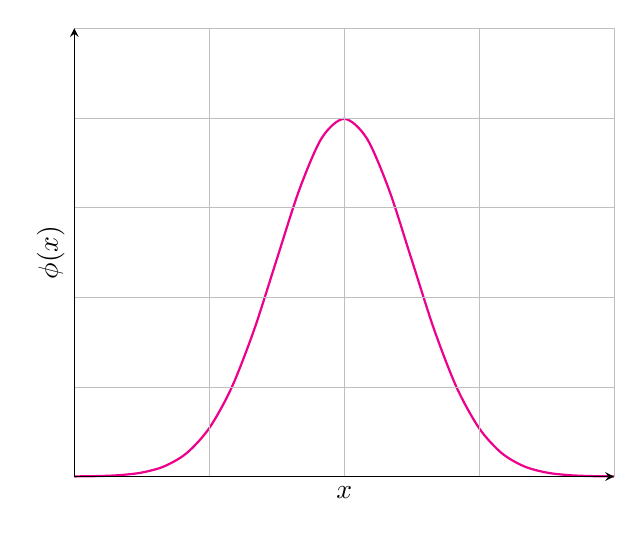
\begin{tikzpicture}
            \begin{axis}[
                xlabel=$x$,
                ylabel=$\phi(x)$,
                xmin=-4, xmax=4,
                ymin=0, ymax=0.5,
                axis lines=left,
                grid=both,
                grid style={line width=.1pt, draw=gray!10},
                major grid style={line width=.2pt,draw=gray!50},
                ticks=none,
                enlargelimits=false,
                clip=false,
                axis on top,
                every axis plot/.append style={thick},
            ]

            \addplot [magenta, smooth, domain=-4:4] {exp(-x^2 / 2) / sqrt(2*pi)};

            \end{axis}
            \end{tikzpicture}
            \item A continuous random variable is \textbf{normally distributed}, or has a \textbf{normal probability distribution}, if its relative frequency histogram has the shape of a normal curve.
            \item \textbf{Inflection Points:} On a bell shaped curve (normal curve), the graph has two inflection points. At $\mu \pm \sigma$, these points are where the graph shifts from increasing at an increasing rate, to increasing at a decreasing rate
      \end{itemize}
      \pagebreak \bigbreak \noindent 
      \textbf{\textit{\underline{Use the Uniform Probability Distribution:}}}
      \bigbreak \noindent 
      Assume that United Parcel Service is supposed to deliver a package to your front door and the arrival time is somewhere between 10 AM and 11 AM. Let the random variable $X$ represent the time from 10 AM when the delivery is supposed to take place.
      \bigbreak \noindent 
    The delivery could be at 10 AM ($x=0$) or at 11 AM ($x=60$), with all one-minute intervals of time between $x=0$ and $x=60$ equally likely. That is to say, your package is just as likely to arrive between 10:15 and 10:16 as it is to arrive between 10:40 and 10:41.
    \bigbreak \noindent 
    The random variable $X$ can be any value in the interval from 0 to 60, that is, $0 \leq X \leq 60$. Because any two intervals of equal length between 0 and 60, inclusive, are equally likely, the random variable $X$ is said to follow a \textbf{uniform probability distribution}.
    \bigbreak \noindent 
    When computing probabilities for discrete random variables, we usually substitute the value of the random variable into a formula.
    \bigbreak \noindent 
    Things are not as easy for continuous random variables. Because an infinite number of outcomes are possible for continuous random variables, the probability of observing one particular value is zero. In the UPS example, the probability that the package arrives exactly 12.9438823 minutes after 10 AM is zero. This result is based on classical probability: there is one way to observe 12.9438823, and there are an infinite number of possible values between 0 and 60. To resolve this problem, we compute probabilities of continuous random variables over an interval of values. For example, we might compute the probability that your package arrives between $x=10$ minutes and $x=15$ minutes after 10 AM. To find probabilities for continuous random variables, we use probability density functions. 

    \bigbreak \noindent 
    \textit{Uniform Density Function for UPS example:}
    % \begin{figure}[ht]
    %     \centering
    %     \incfig{figaro}
    %     \label{fig:figaro}
    % \end{figure}
    \bigbreak \noindent 
    The graph illustrates the properties for the "time" example. Notice the area of the rectangle is one and the graph is greater than or equal to zero for all $x $ between 0 and 60, inclusive
    \bigbreak \noindent 
    Because the area of a rectangle is $l\cdot h $, and the width of the rectangle is 60, the height must be $\frac{1}{60}$
    \bigbreak \noindent 
    \nt{Values of the random variable $X $ less than 0 or greater than 60 are impossible, thus the equation must be zero for $X $ less than 0 or greater than 60.}

    \pagebreak \bigbreak \noindent 
    \textbf{Area as a Probability:}
    \bigbreak \noindent 
    The probability of choosing a time that is between 15 and 30 seconds after the minute is the area under the uniform density function.
    \bigbreak \noindent 
    % \begin{figure}[ht]
    %     \centering
    %     \incfig{figaro2}
    %     \label{fig:figaro2}
    % \end{figure}

    \bigbreak \noindent \bigbreak \noindent 
    \textbf{\textit{\underline{Graph a Normal Curve}}}
    \bigbreak \noindent 
    When describing a uniform random variable using a probability distribution, a rectangle is used to find probabilities of observing an interval of numbers (such as 10 to 20 minutes after 10 AM). However, not all continuous random variables follow a uniform distribution. For example, continuous random variables such as IQ scores and birth weights of babies have distributions that are symmetric and bell-shaped. Consider the histograms in Figure 1, which represent the IQ scores of 10,000 randomly selected adults. Notice that as the class width of the histogram decreases, the histogram becomes closely approximated by the smooth red curve. For this reason, we can use the curve to model the probability distribution of this continuous random variable.
    \bigbreak \noindent 
    \textit{Figure:}
% \begin{figure}[ht]
%     \centering
%     \incfig{normalcurve}
%     \label{fig:normalcurve}
% \end{figure}

    \pagebreak \bigbreak \noindent 
    \textbf{\textit{\underline{State the Properties of the Normal Curve:}}}
    \bigbreak \noindent 
    The normal probability density function satisfies all the requirements of probability distributions. Now we list the properties of the normal density curve. The video explains the properties.
    \begin{enumerate}
    \item Because mean = median = mode, the normal curve has a single peak and the highest point occurs at $x=\mu$.
    \item The normal curve has inflection points at $\mu-\sigma$ and $\mu+\sigma$.
    \item The area under the normal curve is 1.
    \item The area under the normal curve to the right of $\mu$ equals the area under the normal curve to the left of $\mu$, which equals 0.5.
    \item As $x$ increases without bound (gets larger and larger), the graph approaches, but never reaches, the horizontal axis. As $x$ decreases without bound (gets more and more negative), the graph approaches, but never reaches, the horizontal axis.
    \item The Empirical Rule:
    \begin{itemize}
        \item Approximately 68\% of the area under the normal curve is between $x=\mu-\sigma$ and $x=\mu+\sigma$.
        \item Approximately 95\% of the area is between $x=\mu-2\sigma$ and $x=\mu+2\sigma$.
        \item Approximately 99.7\% of the area is between $x=\mu-3\sigma$ and $x=\mu+3\sigma$.
    \end{itemize}
    \end{enumerate}

    \bigbreak \noindent \bigbreak \noindent 
    \textbf{\textit{\underline{Explain the Role of Area in the Normal Density Function:}}}
    \bigbreak \noindent 
    \textbf{Area under a Normal Curve}
    \bigbreak \noindent 
    Suppose that a random variable $X$ is normally distributed with mean $\mu$ and standard deviation $\sigma$. The area under the normal curve for any interval of values of the random variable $X$ represents either
    \bigbreak \noindent 
    \begin{itemize}
        \item The proportion of the population with the characteristic described by the interval of values,
        \smallbreak
        or
        \item The probability that a randomly selected individual from the population will have the characteristic described by the interval of values.
    \end{itemize}

    \pagebreak 
    \phantomsection
    \addcontentsline{toc}{subsection}{7.2: Applications of the Normal Distribution}
    \subsection*{7.2: Applications of the Normal Distribution}
    \bigbreak \noindent 
    \textbf{\textit{\underline{Learning Objectives For This Section:}}}
    \begin{enumerate}
        \item \textbf{Find and Interpret the Area under a Normal Curve}
        \item \textbf{Find the Value of a Normal Random Variable}
    \end{enumerate}
    \bigbreak \noindent 
    \textbf{Vocab:}
    \begin{itemize}
        \item If a normal random variable X has a mean different from 0 or a standard deviation different from 1, we can transform X into a \textbf{standard normal random variable Z} whose mean is 0 and standard deviation is 1. 
    \end{itemize}
    \bigbreak \noindent 

    \pagebreak \bigbreak \noindent 
    \textbf{\textit{\underline{Find and Interpret the Area under a Normal Curve}}}
    \bigbreak \noindent 
    We use z-scores to find the area under a normal curve by hand. Recall that the z-score allows us to transform a random variable X with mean $\mu$ and standard deviation $\sigma $ into a random variable Z with mean 0 and standard deviation 1.
    \bigbreak \noindent 
    \textbf{Standardizing a Normal Random Variable:}
    \bigbreak \noindent 
    Suppose that the random variable $X$ is normally distributed with mean $\mu$ and standard deviation $\sigma$.
    \bigbreak \noindent 
    Then the random variable 
    \begin{align*}
        Z = \frac{X - \mu}{\sigma}
    .\end{align*}
    is normally distributed with mean $\mu = 0$ and standard deviation $\sigma = 1$.
    \bigbreak \noindent 
    The random variable $Z$ is said to have the \textbf{standard normal distribution.}

    \bigbreak \noindent 
    Consider an example:
    \bigbreak \noindent 
    IQ scores can be modeled by a normal distribution with $\mu = 100 $ and $\sigma = 15$ Suppose a person has an IQ of 120
    \bigbreak \noindent 
    \textit{Figure:}
    \bigbreak \noindent 
    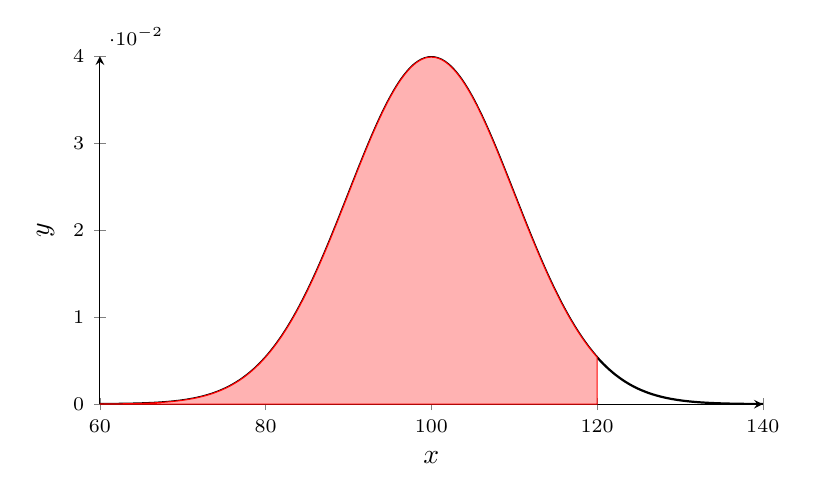
\begin{tikzpicture}
      \begin{axis}[
        width=10cm,
        height=6cm,
        axis lines=left,
        xlabel=$x$,
        ylabel=$y$,
        xmin=60,
        xmax=140,
        ymin=0,
        ymax=0.04,
        xtick={60,80,100,120,140},
        % ytick={0,0.01,0.02,0.03,0.04},
        % yticklabels={0,0.01,0.02,0.03,0.04},
        tick label style={font=\scriptsize},
        samples=100,
        smooth,
        domain=60:140,
      ]
      
      % Bell-shaped curve
      \addplot[black, fill=none, thick] {exp(-((x-100)^2)/(2*10^2))/(10*sqrt(2*pi))};
      
      % Red shaded area
      \addplot[red, fill=red!30, domain=60:120] {exp(-((x-100)^2)/(2*10^2))/(10*sqrt(2*pi))} \closedcycle;
      
      \end{axis}
    \end{tikzpicture}
    \bigbreak \noindent 
        Now we can transform this into a standard normal (Z distribution)
        \begin{align*}
            Z = \frac{120-100}{15} \\
            = 1.33
        .\end{align*}
        \bigbreak \noindent 
        \textit{Figure:}
        \bigbreak \noindent 
        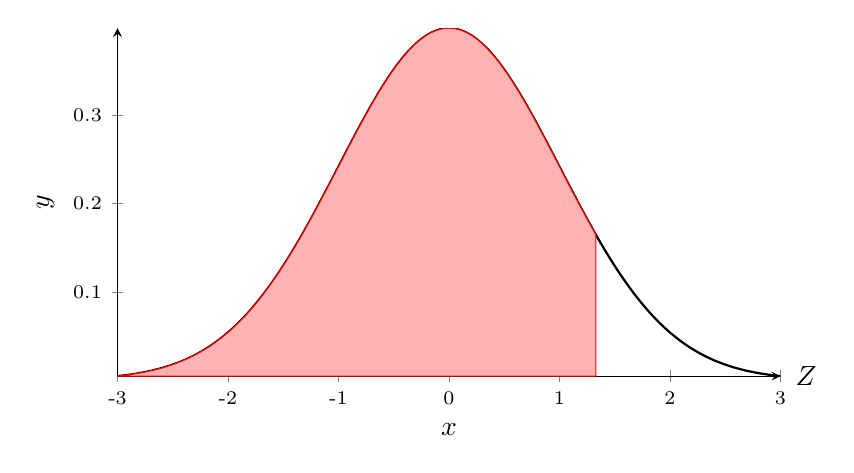
\begin{tikzpicture}
      \begin{axis}[
        width=10cm,
        height=6cm,
        axis lines=left,
        xlabel=$x$,
        ylabel=$y$,
        xtick={-3, -2, -1, 0, 1, 2, 3},
        xticklabels={-3, -2, -1, 0, 1, 2, 3},
        % ytick={0, 0.2, 0.4, 0.6, 0.8, 1.0},
        % yticklabels={0, 0.2, 0.4, 0.6, 0.8, 1.0},
        tick label style={font=\scriptsize},
        samples=100,
        smooth,
        domain=-3:3,
      ]
      
      % Bell-shaped curve
      \addplot[black, fill=none, thick] {exp(-x^2/2)/(sqrt(2*pi))};
      
      % Red shaded area
      \addplot[red, fill=red!30, domain=-3:1.33] {exp(-x^2/2)/(sqrt(2*pi))} \closedcycle;
      
      \end{axis}
      \node[anchor=east] at (9,0) {$Z$};
    \end{tikzpicture}
    \bigbreak \noindent 
    Then by looking at the Table, we can determine the area in the red shaded region. Which is .9082. From this we can also determine that the area in the red region of our original distribution is also .9082

    \bigbreak \noindent \bigbreak \noindent 
    \textbf{Finding an interpreting Area under a Normal Curve With Statcrunch:}
    \begin{enumerate}
        \item Stat $> $ Calculators $> $ Normal 
        \item Input Mean
        \item Input Standard Deviation
        \item Input X
        \item Compute
    \end{enumerate}
    
    \bigbreak \noindent \bigbreak \noindent 
    \textbf{\textit{\underline{Find the Value of a Normal Random Variable:}}}
    \bigbreak \noindent 
    Often, we do not want to find the proportion, probability, or percentile given a value of a normal random variable. Rather, we want to find the value of a normal random variable that corresponds to a certain proportion, probability, or percentile. For example, we might want to know the height of a 3-year-old girl who is at the 20th percentile. Or we might want to know the scores on a standardized exam that separate the middle 90\% of scores from the bottom and top 5\%.

    \bigbreak \noindent 
    \begin{mdframed}
        \textbf{Example: The heights of a pediatrician's 3-year-old females are approximately normally distributed, with mean 38.72 inches and standard deviation 3.17 inches. Find the height of a 3-year-old female at the $20^{th} $ percentile.}
        \bigbreak \noindent 
        \textbf{Approach:}
        \bigbreak \noindent 
        Use .2 in Statcrunch steps mentioned previously as what P(X) is equal to.
    \end{mdframed}
    \bigbreak \noindent 
    \begin{mdframed}
        \textbf{Example: The mean incubation time of fertilized eggs is  days. Suppose the incubation times are approximately normally distributed with a standard deviation of  day. Determine the incubation times that make up the middle 97\%}
        \bigbreak \noindent 
        \textbf{Solution:}
        \bigbreak \noindent 
        So in statcrunch, we will use values 0.05, and 0.97
    \end{mdframed}

    \textbf{Important Notation For the Future:}
  \bigbreak \noindent 
  The notation $z_{\alpha}$ (pronounced "z sub alpha") is the z-score such that the area under the standard normal curve to the right of $z_{\alpha}$ is $\alpha$. 
  \bigbreak \noindent 
  \begin{mdframed}
    \textbf{Example: Find the value of $Z_{0.21} $}
    \bigbreak \noindent 
    \textbf{Solution:}
    So we want to find the area to the right of 0.21, in statcrunch:
    \begin{enumerate}
      \item Stat $> $ Calculator $> $ Normal
      \item Mean: 0 
      \item Std. Dev: 1
      \item $P(x \geq 0) = 0.21$
      \item Compute!
    \end{enumerate}
  \end{mdframed}


  \pagebreak 
  \phantomsection
  \addcontentsline{toc}{subsection}{7.3: Assessing Normality}
  \subsection*{7.3 Assessing Normality}
  \bigbreak \noindent 
  \textbf{\textit{\underline{Learning Objectives For This Section:}}}
  \begin{enumerate}
      \item \textbf{Use Normal Probability Plots to Assess Normality}
  \end{enumerate}
  \bigbreak \noindent 
  \textbf{Vocab:}
  \begin{itemize}
      \item A \textbf{normal probability plot} is a graph that plots observed data versus normal scores. 
      \item A \textbf{normal score} is the expected z-score of the data value, assuming that the distribution of the random variable is normal. The expected z-score of an observed value depends on the number of observations in the data set.
  \end{itemize}

  \pagebreak \bigbreak \noindent 
  \textbf{\textit{\underline{Use Normal Probability Plots to Assess Normality:}}}
  \bigbreak \noindent 
  Up to this point, we have said that a random variable X is normally distributed, or at least approximately normal, provided the histogram of the data is symmetric and bell-shaped. This works well for large data sets, but the shape of a histogram drawn from a small sample of observations does not always accurately represent the shape of the population. For this reason, we need additional methods for assessing the normality of a random variable X when we are looking at a small set of sample data.
  \bigbreak \noindent 
  \textbf{Drawing a Normal Probability Plot by Hand:}
  \begin{enumerate}
      \item Arrange the data in ascending order.
      \item Compute:
          \begin{align*}
             f_{i} = \frac{i-0.375}{n+0.25} 
          .\end{align*}
          where $i $ is the index (the position of the data value in the ordered list) and $n$ is the number of observations. The expected proportion of observations less than or equal to the $i^{th} $ data value is $f_{i}$.
      \item Find the z-score corresponding to $f_{i} $ from Table V.
    \item Plot the observed values on the horizontal axis and the corresponding expected z-scores on the vertical axis.
  \end{enumerate}
  \bigbreak \noindent 
  The idea behind finding the expected z-score is, if the data come from a normally distributed population, we could predict the area to the left of each data value. The value of $f_i$ represents the expected area to the left of the $i$th observation when the data come from a population that is normally distributed. For example, $f_1$ is the expected area to the left of the smallest data value, $f_2$ is the expected area to the left of the second-smallest data value, and so on.
  \bigbreak \noindent 
  Values of normal random variables and their z-scores are linearly related ($x = \mu + z\sigma$), so a plot of observations of normal variables against their expected z-scores will be linear. We conclude the following:
  \bigbreak \noindent 
    If sample data are taken from a population that is normally distributed, a normal probability plot of the observed values versus the expected z-scores will be approximately linear.
    \bigbreak \noindent 
    It is difficult to determine whether a normal probability plot is "linear enough." However, we can use a procedure based on the research of S. W. Looney and T. R. Gulledge in their paper "Use of the Correlation Coefficient with Normal Probability Plots," published in the American Statistician. Basically, if the linear correlation coefficient between the observed values and expected z-scores is greater than the critical value found in Table VI, then it is reasonable to conclude that the data could come from a population that is normally distributed.
    \bigbreak \noindent 
    Normal probability plots are typically drawn using technology (graphing calculators or statistical software). However, it is worthwhile to go through an example that demonstrates how to draw a normal probability plot by hand to better understand the results supplied by technology.

    \pagebreak \bigbreak \noindent 
    \textbf{Drawing a Normal Probability Plot Using Statcrunch}
    \bigbreak \noindent 
    \begin{enumerate}
        \item Graph $> $ QQ plot
        \item Select Column
        \item Select Correlation Statistic
        \item Compute
    \end{enumerate}

    \pagebreak 
    \begin{center}
        \phantomsection
        \addcontentsline{toc}{section}{Chapter 8}
        \section*{Chapter 8}
    \end{center}
    \line(1,0){490}
    \bigbreak \noindent 
    \phantomsection
    \addcontentsline{toc}{subsection}{8.1 Distribution of the Sample Mean}
    \subsection*{8.1 Distribution of the Sample Mean}
    \bigbreak \noindent 
    \textbf{\textit{\underline{Learning Objectives For This Section:}}}
    \begin{enumerate}
        \item \textbf{Describe the Distribution of the Sample Mean: Normal Population}
        \item \textbf{Describe the Distribution of the Sample Mean: Non-normal Population}
    \end{enumerate}
    \bigbreak \noindent 
    \textbf{Vocab:}
    \begin{itemize}
        \item The \textbf{sampling distribution} of a statistic is a probability distribution for all possible values of the statistic computed from a sample of size $n $
        \item The \textbf{sampling distribution of the sample mean} $\overline{x} $ is the probability distribution of all possible values of the random variable $\overline{x} $ computed from a sample of size $n$ from a population with mean $\mu $ and standard deviation $\sigma $.
        \item The standard deviation of the sampling distribution of $\overline{x} $, $\sigma_{\overline{x}} $, is called the \textbf{standard error} of the mean.
            \textbf{Note:} As the sample size $n $ increases, the standard error of the mean \textbf{decreases} 
        \item \textbf{The Central Limit Theorem:} Regardless of the shape of the underlying population, the sampling distribution of $\overline{x} $  becomes approximately normal as the sample size, $n $, increases
    \end{itemize}
    \bigbreak \noindent 
    \bigbreak \noindent 
    \textbf{Formulas:}
    \begin{itemize}
        \item \textbf{Mean of sampling distribution}
            \begin{align*}
                \mu_{\overline{x}} = \mu
            .\end{align*}
        \item \textbf{Standard Deviation of sampling distribution}
            \begin{align*}
                \sigma_{\overline{x}} = \sqrt{\frac{N-n}{N-1}} \cdot \frac{\sigma}{\sqrt{n}}
            .\end{align*}
        \item \textbf{finite population correction factor}
            \begin{align*}
                \sqrt{\frac{N-n}{N-1}}
            .\end{align*}
    \end{itemize}
    \pagebreak \bigbreak \noindent 
    \textbf{\textit{\underline{Introduction: The idea that the sample mean is a \textbf{random variable}}}}
    \bigbreak \noindent 
    Suppose the government wanted to determine the mean income of all U.S. households. One approach the government could take is literally to survey each U.S. household to determine the population mean. This would be a very expensive and time-consuming survey.
    \bigbreak \noindent 
    A second approach the government could (and does) take is to survey a random sample of U.S. households and use the results to estimate the mean income of all households. The Current Population Survey is administered to approximately 60,000 randomly selected households each month. Among the many questions on the survey, respondents are asked to report the income of each individual in the household. From this information, the federal government obtains a sample mean U.S. household income. For example, in 2015, the mean annual U.S. household income was approximately $\overline{x}$=\$79,263. The government might infer from this survey that the mean annual household income of all U.S. households in 2015 was \$\mu $=$79,263.
    \bigbreak \noindent 
    The households in the Current Population Survey were determined by chance (random sampling). A second random sample of households would likely lead to a different sample mean, such as $\overline{x} $=\$78,518, and a third random sample of households would likely lead to a third sample mean, such as $\overline{x} $=\$79,081. Because the households selected will vary from sample to sample, the sample mean of household income will also vary from sample to sample. For this reason, \textbf{the sample mean is a random variable}; so it has a probability distribution. Our goal in this section is to describe the distribution of the sample mean. Remember, when we describe a distribution, we do so in terms of its shape, center, and spread.
    \bigbreak \noindent 
    \textbf{Steps for Determining the Sampling Distribution of the Sample Mean}
    \bigbreak \noindent 
    \begin{enumerate}
        \item Obtain a simple random sample of size $n $
        \item Compute the sample mean.
        \item Assuming that we are sampling from a finite population, repeat Steps 1 and 2 until all distinct simple random samples of size $n $ have been obtained.
    \end{enumerate}
    \bigbreak \noindent 
    \nt{Once a particular sample is obtained, it cannot be obtained a second time.}
        
    \pagebreak \bigbreak \noindent 
    \textbf{\textit{\underline{Describe the Distribution of the Sample Mean: Normal Population}}}
    \bigbreak \noindent 
    \textbf{Key points:}
    \begin{itemize}
        \item \textbf{Shape:} the shape of the distribution of the sample mean becomes approximately normal as the sample size $n $ increases, regardless of the shape of the underlying population
        \item \textbf{Center:} The mean of the distribution of the sample mean will equal the mean of the parent population, $\mu_{\overline{x}} = \mu $.
        \item \textbf{Spread:} The standard devitaino of the distribution of the sample mean is less than the standard deviation of the population. And, the larger the sample size, $n $, the smaller the standard deviation of the distribution of the sample mean.
    \end{itemize}
    we conclude that the mean of the distribution of the sample mean, $\overline{x} $ equals the mean of the parent population and as the sample size $n $ increases, the standard deviation of the distribution of $\overline{x} $ decreases. Although the proof is beyond the scope of this course. 
    \bigbreak \noindent 
    \textbf{The Mean and Standard Deviation of the Sampling Distribution of $\overline{x} $:}
    \bigbreak \noindent 
    Suppose that a simple random sample of size $n $ is drawn from a population with mean $\mu$ and standard deviation $\sigma$. The sampling distribution of $\bar{x}$ has mean $\mu_{\bar{x}} = \mu$ and standard deviation $\sigma_{\bar{x}} = \frac{\sigma}{\sqrt{n}}$. The standard deviation of the sampling distribution of $\bar{x}$, $\sigma_{\bar{x}}$, is called the standard error of the mean.
    \bigbreak \noindent 
    \textbf{Note:} Technically, we assume that we are drawing a simple random sample from an infinite population. For populations of finite size \(N\), 
    \begin{align*}
        \sigma_{\overline{x}} = \sqrt{\frac{N-n}{N-1}} \cdot \frac{\sigma}{\sqrt{n}}
    .\end{align*}
     However, if the sample size is less than 5\% of the population size $n < 0.05N$, the effect of $\sqrt{\frac{N - n}{N - 1}}$ (the finite population correction factor) can be ignored without significantly affecting the result.
     \bigbreak \noindent 
     \textbf{In summary:}
     \bigbreak \noindent 
     Say we have a set of data, Where each row represents a sample of the population, we can compute $\overline{x} $ for each row of data, and then with this new row of $\overline{x}$'s, we can compute $\mu_{\overline{x}}$ and $\sigma_{\overline{x}}$

     \pagebreak \bigbreak \noindent 
     Now that we can find the mean and standard deviation for any sampling distribution of x¯¯¯, we can concentrate on the shape of the distribution. In the simulations from the video, both histograms of the 2000 different sample means appear to be normal. Recall that the population from which the sample was drawn was also normal. This result leads us to believe that if the population is normal, then the distribution of the sample mean is also normal.
     \bigbreak \noindent 
     \textbf{The Shape of the Sampling Distribution of $\overline{x} $ If $X$ Is Normal}
     \bigbreak \noindent 
     If a random variable $X $ is normally distributed, the distribution of the sample mean, $\overline{x} $, is normally distributed.
     \bigbreak \noindent 
     \begin{mdframed}
       \textbf{Example: The IQ, $X$, of humans is approximately normally distributed with mean $\mu=100$ and standard deviation $\sigma=15$. Compute the probability that a simple random sample of size $n=10$ results in a sample mean greater than $110$. That is, compute $P(\bar{x}>110)$.}
       \bigbreak \noindent 
       \textbf{Approach}
       \bigbreak \noindent 
        The random variable $X$ is normally distributed, so the sampling distribution of $\bar{x}$ will also be normally distributed. Verify the sample size is less than 5\% of the population size (the independence requirement). The mean of the sampling distribution is $\mu_{\bar{x}}=\mu$, and its standard deviation is $\sigma_{\bar{x}}=\frac{\sigma}{\sqrt{n}}$. To find the probability by hand, convert the sample mean $\bar{x}=110$ to a z-score and then find the area under the standard normal curve to the right of this z-score, or use technology to find the area.
        \bigbreak \noindent 
        \textbf{Solution:}
        \bigbreak \noindent 
        So we find $\mu_{\overline{x}}$ and $\sigma_{\overline{x}}:$
        \begin{align*}
            \mu_{\overline{x}} = \mu = 100 \\
            \sigma_{\overline{x}} = \frac{s}{\sqrt{n}} = \frac{15}{\sqrt{10}} = 4.7434
        .\end{align*}
        \bigbreak \noindent 
        Now in stat crunch:
        \begin{itemize}
            \item Stat $> $ Calculators $> $ Normal
            \item Input $\mu_{\overline{x}}$ as the mean
            \item Input $\sigma_{\overline{x}}$ as the standard deviation
            \item Input $P(x \geq 110) $
            \item Compute
        \end{itemize}
        \bigbreak \noindent 
        And we end up with
        \begin{align*}
            .0.175
        .\end{align*}
     \end{mdframed}

     \pagebreak \bigbreak \noindent 
     \textbf{\textit{\underline{Describe the Distribution of the Sample Mean: Non-normal Population}}}
     \bigbreak \noindent 
     \begin{enumerate}
         \item \textbf{Shape:} The shape of the distribution of the sample mean becomes approximately normal as the sample size $n $ increases, regardless of the shape of the underlying population.
        \item \textbf{Center:} The mean of the distribution of the sample mean will equal the mean of the parent population, $\mu_{\overline{x}} = \mu$
        \item \textbf{Spread:} The standard deviation of the distribution of the sample mean is less than the standard deviation of the population, And, the larger the sample size, $n $, the smaller the standard deviation of the distribution of the sample mean.
     \end{enumerate}
     \bigbreak \noindent 
     There are two key concepts to understand from the above points:
     \begin{enumerate}
         \item The mean of the sampling distribution of the sample mean is equal to the mean of the underlying population. That is, $\mu_{\overline{x} = \mu} $ regardless of the size of the sample. The standard deviation of the sampling distribution of the sample mean is $\sigma_{\overline{x}} = \frac{\sigma}{\sqrt{n}} $, regardless of the size of the sample.
        \item The shape of the distribution of the sample mean becomes approximately normal as the sample size $n$ increases, regardless of the shape of the underlying population.
        \hspace{\parindent}  We formally state point 2 as the Central Limit Theorem.
     \end{enumerate}






\end{document}
